% Provenance (never printed): see sources/outline_sources.md (Year 1: stress and
% principal stresses in 2D; strain; pure and simple shear; elastic, brittle and ductile
% behaviour; the strength envelope of the lithosphere). Strength envelopes from
% figdata/bachelor-1/strength_envelope.py (Byerlee 1975; flow laws of Gleason and Tullis
% 1995 and Hirth and Kohlstedt 2003 as compiled by Lopez-Sanchez; geotherms of ch. 10);
% exercise and problem values in the Book 3 scratch calculator calc/ch16.py. Traction,
% shear stress, the stress and strain tensors, Hooke's law, Young's modulus and viscosity
% belong to the physics series and are recalled, never defined (sync 1 ruling).
\chapter{Tensão, deformação e reologia}\label{ch:b1:stress-strain-rheology}

Nos anos 1960, fluido residual bombeado por um poço de descarte na Rocky Mountain Arsenal, perto de Denver, espalhou-se pelo embasamento cristalino fraturado entre \qty{3.7}{km} e \qty{7.0}{km} abaixo da superfície, e terremotos se seguiram. Eles ficaram dentro da parte da rocha onde a pressão do fluido havia subido em mais de cerca de \qty{3.2}{MPa}.
% ledger: hb81:denver
Meio século depois, a mesma coisa aconteceu em escala maior em Oklahoma, onde a água salgada trazida à superfície com o petróleo e o gás é bombeada de volta ao subsolo. Em todo o estado e em seus arredores, os terremotos de magnitude 3 ou mais somavam de um a cinco por ano entre 2005 e 2008, depois \num{20} em 2009, \num{585} em 2014 e \num{888} em 2015, mais de dois por dia; abalos de magnitude 5.7 e 5.8 sacudiram Prague, em 2011, e Pawnee, em 2016. Apenas quatro poços de descarte de grande volume poderiam explicar um quinto dos terremotos do centro dos Estados Unidos, e provocar alguns a mais de \qty{30}{km} de distância.
% ledger: usgs:oklahoma-rate, usgs:prague-pawnee, keranen:oklahoma
A água não empurrou nada para o lado; apenas elevou a \omterm{def:b1:stress-strain-rheology:lithostatic}{pressão do fluido nos poros} da rocha. Por que isso faria uma falha deslizar? A resposta exige três ideias, que são o assunto deste capítulo: a tensão sobre um plano dentro de uma rocha, a condição sob a qual o plano cede, e o fato de que a \omterm{def:b1:stress-strain-rheology:lithostatic}{pressão do fluido nos poros} atua contra a força que comprime os dois lados um contra o outro. Com elas, e com uma lei de fluência para rocha quente, podemos traçar a resistência de toda a \omterm{def:b1:layered-earth:lithosphere}{litosfera} em função da profundidade.

\begin{recall}
Uma força distribuída sobre uma superfície atua por sua força por unidade de área, em pascals; a pressão em um fluido em repouso cresce com a profundidade como $\rho g z$ (livros de física). Uma mola, e um sólido em pequenas deformações, obedecem à lei de Hooke: a deformação é proporcional à tensão, com o módulo de Young como constante; um fluido viscoso resiste em proporção à sua taxa de cisalhamento, com a viscosidade como constante. O volume do Livro 5 dos livros de física descreve tensão e deformação em três dimensões com tensores; este capítulo precisa apenas de dois. Uma matriz simétrica $2\times2$ tem dois autovalores reais e dois autovetores perpendiculares (matemática, primeiro ano). As geotermas de \cref{ch:b1:heat-budget} dão a temperatura em profundidade; falhas foram estudadas no Livro 1, 7º ano.
\end{recall}

\section{Tensão em duas dimensões}\label{sec:b1:stress-strain-rheology:stress}

Corte uma rocha, em pensamento, ao longo de uma pequena superfície plana. A rocha de um lado pressiona a rocha do outro com uma força, e a força por unidade de área é a tração sobre essa superfície, na palavra dos livros de física. Sua direção não é, em geral, a direção da normal à superfície.

\begin{definition}[Tensão normal]\label{def:b1:stress-strain-rheology:stress}
Sobre um plano através de um ponto de uma rocha, a força por unidade de área que a rocha de um lado exerce sobre a do outro tem uma componente ao longo da normal ao plano, a \emph{tensão normal}\index{tensão normal} $\sigma_n$, e uma componente ao longo do plano, a tensão de cisalhamento $\tau$. Nas ciências da Terra, a tensão normal é contada como positiva quando comprime.
\end{definition}

A convenção de sinal é a oposta à do engenheiro. Ela foi escolhida porque quase toda tensão no sólido terrestre é uma compressão: o peso da rocha acima pressiona tudo o que está abaixo dela.

Trabalhamos em um plano vertical, com um eixo $x$ horizontal e um eixo $y$. Sobre um plano perpendicular a $x$, a \omterm{def:b1:stress-strain-rheology:stress}{tensão normal} é $\sigma_{xx}$ e a de cisalhamento $\sigma_{xy}$; sobre um plano perpendicular a $y$, são $\sigma_{yy}$ e $\sigma_{yx}$. As duas tensões de cisalhamento são iguais: em um pequeno quadrado, as forças de cisalhamento nos lados verticais formam um binário de momento $\sigma_{xy}a\cdot a$ para um lado $a$, e as dos lados horizontais, um binário $\sigma_{yx}a\cdot a$ girando no sentido oposto, e o quadrado giraria se elas fossem diferentes. Assim, três números descrevem a tensão em um ponto, e bastam para dá-la em todo plano.

\begin{proposition}[Tensão sobre um plano inclinado]\label{prop:b1:stress-strain-rheology:transformation}
Seja um plano de normal unitária $\vec n = (\cos\theta, \sin\theta)$, formando o ângulo $\theta$ com o eixo $x$, e seja $\vec m = (-\sin\theta, \cos\theta)$ o vetor unitário ao longo do plano. As tensões normal e de cisalhamento sobre ele são
\begin{align*}
  \sigma_n &= \sigma_{xx}\cos^2\theta + 2\sigma_{xy}\sin\theta\cos\theta + \sigma_{yy}\sin^2\theta
           = \frac{\sigma_{xx}+\sigma_{yy}}{2} + \frac{\sigma_{xx}-\sigma_{yy}}{2}\cos2\theta + \sigma_{xy}\sin2\theta, \\
  \tau     &= (\sigma_{yy}-\sigma_{xx})\sin\theta\cos\theta + \sigma_{xy}(\cos^2\theta - \sin^2\theta)
           = -\frac{\sigma_{xx}-\sigma_{yy}}{2}\sin2\theta + \sigma_{xy}\cos2\theta ,
\end{align*}
com $\tau$ contada positiva ao longo de $\vec m$.
\end{proposition}

\begin{proof}
Recorte um pequeno prisma, como na figura abaixo: uma face inclinada de área $A$ com a normal externa $\vec n$, uma face vertical de área $A\cos\theta$ e uma face horizontal de área $A\sin\theta$, por unidade de comprimento na terceira direção. Seu peso e sua inércia crescem como seu volume, que diminui mais depressa que suas faces; para um prisma pequeno o bastante, as forças sobre as faces devem se equilibrar por si mesmas. Sendo a compressão positiva, a rocha de fora empurra a face vertical com a força $A\cos\theta\,(\sigma_{xx}, \sigma_{xy})$ e a face horizontal com $A\sin\theta\,(\sigma_{xy}, \sigma_{yy})$; sobre a face inclinada ela empurra com $-A(\sigma_n\vec n + \tau\vec m)$. A soma é zero:
\[
  \sigma_n\vec n + \tau\vec m = \cos\theta\,(\sigma_{xx}, \sigma_{xy}) + \sin\theta\,(\sigma_{xy}, \sigma_{yy}) .
\]
O produto escalar com $\vec n$ dá $\sigma_n$, com $\vec m$ dá $\tau$, pois $\vec n\cdot\vec m = 0$. As segundas formas seguem de $\cos^2\theta = (1+\cos2\theta)/2$, $\sin^2\theta = (1-\cos2\theta)/2$ e $2\sin\theta\cos\theta = \sin2\theta$.
\end{proof}

\begin{omfigure}
\begin{tikzpicture}[>={Stealth[length=5pt]}, font=\small]
% theta = 35 deg, hypotenuse L = 4.5: a = L cos(theta), b = L sin(theta)
\pgfmathsetmacro{\th}{35}
\pgfmathsetmacro{\L}{4.5}
\pgfmathsetmacro{\a}{\L*cos(\th)}
\pgfmathsetmacro{\b}{\L*sin(\th)}
\coordinate (O) at (0,0);
\coordinate (A) at (0,\a);
\coordinate (B) at (\b,0);
\coordinate (M) at ($(A)!0.5!(B)$);
\fill[omLithGranite!45] (O) -- (A) -- (B) -- cycle;
\draw[line width=0.8pt] (O) -- (A) -- (B) -- cycle;
% axes
\draw[->, black!70] (-2.6,-1.9) -- (-1.6,-1.9) node[right] {$x$};
\draw[->, black!70] (-2.6,-1.9) -- (-2.6,-0.9) node[above] {$y$};
% face on x = 0 (outward normal -x), area A cos(theta)
\draw[->, line width=1.1pt, omDef] (-1.35,0.5*\a) -- (-0.05,0.5*\a);
\node[omDef, anchor=south] at (-0.95,0.5*\a+0.05) {$\sigma_{xx} A\cos\theta$};
\draw[->, line width=1.1pt, omProp] (-0.25,0.5*\a-1.25) -- (-0.25,0.5*\a-0.25);
\node[omProp, anchor=east] at (-0.3,0.5*\a-0.85) {$\sigma_{xy} A\cos\theta$};
% face on y = 0 (outward normal -y), area A sin(theta)
\draw[->, line width=1.1pt, omDef] (0.68*\b,-1.35) -- (0.68*\b,-0.05);
\node[omDef, anchor=west] at (0.68*\b+0.05,-1.05) {$\sigma_{yy} A\sin\theta$};
\draw[->, line width=1.1pt, omProp] (0.1,-0.25) -- (1.1,-0.25);
\node[omProp, anchor=north east] at (0.9,-0.32) {$\sigma_{xy} A\sin\theta$};
% inclined face, area A, normal n = (cos theta, sin theta)
\draw[->, line width=1.1pt, omThm] ($(M)+(\th:1.5)$) -- ($(M)+(\th:0.05)$);
\node[omThm, anchor=south west, inner sep=1pt] at ($(M)+(\th:1.5)$) {$\sigma_n A$};
\draw[->, line width=1.1pt, omThm!70!black] ($(M)+(\th:0.25)+(\th-90:0.75)$) -- ($(M)+(\th:0.25)+(\th-90:1.75)$);
\node[omThm!70!black, anchor=west] at ($(M)+(\th:0.3)+(\th-90:1.3)$) {$\tau A$};
\draw[->, black!70, dashed] ($(M)+(\th+90:1.25)$) -- ++(\th:1.0) node[pos=1, anchor=south west, inner sep=1pt, text=black] {$\boldsymbol n$};
% angle theta at A, between the face and the y axis
\pic[draw, angle radius=0.75cm, pic text={$\theta$}, angle eccentricity=1.35] {angle = O--A--B};
\end{tikzpicture}
\par\smallskip{\small O equilíbrio de forças sobre um pequeno prisma triangular de rocha. A face inclinada tem área $A$ e normal unitária $\vec n$; as faces vertical e horizontal têm áreas $A\cos\theta$ e $A\sin\theta$. Azul: as forças normais sobre as duas pequenas faces; laranja: as forças de cisalhamento sobre elas; vermelho: as forças normal e de cisalhamento sobre a face inclinada. A compressão é contada como positiva, de modo que toda força normal aponta para dentro do prisma.}
\label{fig:b1:stress-strain-rheology:prism}
\end{omfigure}

\begin{theorem}[Tensões principais]\label{thm:b1:stress-strain-rheology:principal}
Em todo ponto de uma rocha há dois planos perpendiculares nos quais a tensão de cisalhamento é nula. As tensões normais sobre eles são a maior e a menor \omterm{def:b1:stress-strain-rheology:stress}{tensão normal} entre todos os planos que passam pelo ponto,
\[
  \sigma_{1,3} = \frac{\sigma_{xx}+\sigma_{yy}}{2} \pm
  \sqrt{\Bigl(\frac{\sigma_{xx}-\sigma_{yy}}{2}\Bigr)^2 + \sigma_{xy}^2},
  \qquad \tan2\theta_p = \frac{2\sigma_{xy}}{\sigma_{xx}-\sigma_{yy}},
\]
onde $\theta_p$ é o ângulo do eixo $x$ à normal do plano que carrega $\sigma_1$.
\end{theorem}

\begin{proof}
Escreva $c = (\sigma_{xx}+\sigma_{yy})/2$, e escolha $R \ge 0$ e $\theta_p$
com $(\sigma_{xx}-\sigma_{yy})/2 = R\cos2\theta_p$ e
$\sigma_{xy} = R\sin2\theta_p$; então
$R = \sqrt{((\sigma_{xx}-\sigma_{yy})/2)^2 + \sigma_{xy}^2}$ e
$\tan2\theta_p$ é como enunciado. As segundas formas da
\cref{prop:b1:stress-strain-rheology:transformation} tornam-se
\[
  \sigma_n = c + R\cos(2\theta - 2\theta_p), \qquad \tau = -R\sin(2\theta - 2\theta_p).
\]
A \omterm{def:b1:stress-strain-rheology:stress}{tensão normal} é maior, $c + R$, para $\theta = \theta_p$, e menor, $c - R$, para $\theta = \theta_p + \ang{90}$; em ambos, $\tau = 0$. Note também que $\mathrm d\sigma_n/\mathrm d\theta = 2\tau$: a \omterm{def:b1:stress-strain-rheology:stress}{tensão normal} é estacionária exatamente onde a tensão de cisalhamento se anula.
\end{proof}

\begin{definition}[Tensões principais; tensão diferencial]\label{def:b1:stress-strain-rheology:principal}
As \emph{tensões principais}\index{tensões principais} em um ponto são as tensões normais $\sigma_1 \ge \sigma_3$ sobre os dois planos livres de tensão de cisalhamento, e suas direções são as direções principais. Em três dimensões há três, $\sigma_1 \ge \sigma_2 \ge \sigma_3$, sobre três planos perpendiculares. A \emph{tensão diferencial}\index{tensão diferencial} é $\sigma_1 - \sigma_3$, e a tensão média no plano é $(\sigma_1+\sigma_3)/2$.
\end{definition}

Um estado de tensão é mais fácil de ler em suas direções principais. Se medirmos o ângulo $\theta$ a partir da direção de $\sigma_1$ em vez de a partir do eixo $x$, as fórmulas perdem seus últimos termos.

\begin{proposition}[Círculo de Mohr]\label{prop:b1:stress-strain-rheology:mohr}
Sobre um plano cuja normal faz o ângulo $\theta$ com a direção de $\sigma_1$,
\[
  \sigma_n = \frac{\sigma_1+\sigma_3}{2} + \frac{\sigma_1-\sigma_3}{2}\cos2\theta,
  \qquad
  |\tau| = \frac{\sigma_1-\sigma_3}{2}\,|\sin2\theta| .
\]
À medida que $\theta$ gira, o ponto $(\sigma_n, |\tau|)$ percorre a metade superior do círculo de centro $((\sigma_1+\sigma_3)/2,\, 0)$ e raio $(\sigma_1-\sigma_3)/2$, no ângulo $2\theta$ a partir de sua extremidade $\sigma_1$. A maior tensão de cisalhamento, $(\sigma_1-\sigma_3)/2$, atua nos planos a \ang{45} das direções principais.
\end{proposition}

\begin{proof}
Nos eixos principais $\sigma_{xx} = \sigma_1$, $\sigma_{yy} = \sigma_3$ e $\sigma_{xy} = 0$, e a
\cref{prop:b1:stress-strain-rheology:transformation} dá as duas fórmulas. Então
$(\sigma_n - (\sigma_1+\sigma_3)/2)^2 + \tau^2 = ((\sigma_1-\sigma_3)/2)^2$, a equação do círculo; $|\sin2\theta|$ é máximo para $\theta = \ang{45}$.
\end{proof}

O sinal de $\tau$ diz apenas em que sentido os dois lados deslizariam, por isso a metade superior do círculo costuma ser desenhada sozinha. A construção leva o nome do engenheiro Christian Otto Mohr, que também construiu sobre ela um critério de ruptura, que é para onde vamos
(\cref{sec:b1:stress-strain-rheology:rheology}).

\subsection*{Tensão em profundidade}

\begin{definition}[Pressão litostática, pressão do fluido nos poros, tensão efetiva]\label{def:b1:stress-strain-rheology:lithostatic}
À profundidade $z$, o peso da rocha acima, por unidade de área horizontal, é a tensão vertical $\sigma_v = \int_0^z\rho g\,\mathrm dz'$, que é $\rho g z$ em uma camada de densidade uniforme $\rho$. Quando a tensão é a mesma em todas as direções, igual à vertical, a rocha está sob a \emph{pressão litostática}\index{pressão litostática}. A pressão da água, do óleo ou do gás nos poros e fissuras da rocha é a \emph{pressão do fluido nos poros}\index{pressão do fluido nos poros} $P$; ela é hidrostática, $P = \rho_w g z$, quando os poros se conectam à superfície. A \emph{tensão efetiva}\index{tensão efetiva} é a tensão menos a pressão nos poros, $\sigma' = \sigma - P$, em todo plano; $\lambda = P/\sigma_v$ é a razão de pressão nos poros.
\end{definition}

Em uma \omterm{def:b1:layered-earth:layers}{crosta} de densidade \qty{2700}{kg.m^{-3}}, a tensão vertical cresce $2700\times9.81\times1000 = \qty{26.5}{MPa}$ por quilômetro, e a pressão hidrostática nos poros cresce \qty{9.81}{MPa} por quilômetro: $\lambda = 1000/2700 = 0.37$. O fluido dos poros empurra os grãos para longe com a mesma pressão em todas as direções; ele não retira nada da tensão de cisalhamento, mas retira $P$ de toda \omterm{def:b1:stress-strain-rheology:stress}{tensão normal}. Onde os poros são selados, por argila ou sal, por exemplo, o fluido pode carregar parte do peso da rocha acima, e $\lambda$ sobe em direção a 1.

A tensão na \omterm{def:b1:layered-earth:layers}{crosta} não é litostática. Placas empurram e puxam, a \omterm{def:b1:layered-earth:layers}{crosta} se curva, montanhas pesam sobre suas raízes, e as tensões horizontais diferem da vertical. Perto da superfície, que não suporta tensão de cisalhamento, uma direção principal é vertical, como mostra o \cref{ch:b1:faults-folds-fabrics}: $\sigma_v$ é $\sigma_1$, $\sigma_2$ ou $\sigma_3$, e os três casos são as três maneiras como as falhas se movem.

\section{Deformação}\label{sec:b1:stress-strain-rheology:strain}

A tensão é uma causa; a deformação é o que a rocha registra. Um fóssil alongado, um seixo achatado, uma camada encurtada em \omterm{def:b1:geological-maps:fold}{dobras} medem todos uma mudança de forma.

\begin{definition}[Extensão, alongamento, deformação de cisalhamento]\label{def:b1:stress-strain-rheology:strain}
Uma linha de material de comprimento $\ell_0$, deformada até o comprimento $\ell$, tem a \emph{extensão}\index{extensão (deformação)} $e = (\ell - \ell_0)/\ell_0$ e o \emph{alongamento}\index{alongamento} $S = \ell/\ell_0 = 1 + e$; um encurtamento é uma extensão negativa, um alongamento abaixo de 1. Duas linhas de material que eram perpendiculares e agora formam o ângulo $\ang{90} - \psi$ foram cisalhadas pelo ângulo $\psi$, e a \emph{deformação de cisalhamento}\index{deformação de cisalhamento} é $\gamma = \tan\psi$.
\end{definition}

Uma deformação é homogênea quando cada pequena região da rocha se deforma do mesmo modo. A nova posição $\vec x'$ do ponto $\vec x$ é então uma função linear, $\vec x' = F\vec x$, com uma matriz constante $2\times2$ $F$ (e $\det F > 0$, pois a rocha não se vira pelo avesso). Retas continuam retas e retas paralelas continuam paralelas; um quadrado torna-se um paralelogramo, e um círculo torna-se uma elipse.

\begin{proposition}[A elipse de deformação]\label{prop:b1:stress-strain-rheology:ellipse}
Sob a deformação homogênea $\vec x' = F\vec x$, o círculo de raio 1 torna-se uma elipse cujos semieixos são as raízes quadradas $S_1 \ge S_2$ dos autovalores de $FF^{\mathsf T}$, ao longo de seus autovetores perpendiculares. $S_1$ e $S_2$ são os maiores e menores \omterm{def:b1:stress-strain-rheology:strain}{alongamentos} de todas as linhas de material, e a área é multiplicada por $\det F = S_1S_2$.
\end{proposition}

\begin{proof}
O ponto $\vec x = F\vec u$ provém de um ponto $\vec u$ do círculo, $|\vec u| = 1$, logo $|F^{-1}\vec x|^2 = 1$, isto é, $\vec x^{\mathsf T}(FF^{\mathsf T})^{-1}\vec x = 1$. A matriz $B = FF^{\mathsf T}$ é simétrica com autovalores positivos $\lambda_1 \ge
\lambda_2$ ($\vec v^{\mathsf T}B\vec v = |F^{\mathsf T}\vec v|^2 > 0$); em seus autovetores perpendiculares a equação se lê $x_1^2/\lambda_1 + x_2^2/\lambda_2 = 1$, uma elipse de semieixos $\sqrt{\lambda_1}$ e $\sqrt{\lambda_2}$. Uma linha de material ao longo do vetor unitário $\vec u$ tem o \omterm{def:b1:stress-strain-rheology:strain}{alongamento} $|F\vec u|$, e $|F\vec u|^2 = \vec u^{\mathsf T}F^{\mathsf T}F\vec u$ fica entre os autovalores de $F^{\mathsf T}F$, que são os de $FF^{\mathsf T}$. Por fim, $\lambda_1\lambda_2 = \det B = (\det F)^2$.
\end{proof}

\begin{definition}[Elipse de deformação]\label{def:b1:stress-strain-rheology:strain-ellipse}
A \emph{elipse de deformação}\index{elipse de deformação} é a elipse na qual uma deformação homogênea transforma um círculo de raio 1; seus semieixos são os \omterm{def:b1:stress-strain-rheology:strain}{alongamentos} principais $S_1 \ge S_2$, e seus eixos, as direções principais da deformação.
\end{definition}

Duas deformações que alteram a forma de um corpo igualmente podem ser muito diferentes.

\begin{definition}[Cisalhamento puro, cisalhamento simples]\label{def:b1:stress-strain-rheology:shear-types}
Um \emph{cisalhamento puro}\index{cisalhamento puro} é uma deformação homogênea que conserva a área e mantém fixas suas direções principais na rocha: $F = \begin{pmatrix} k & 0 \\ 0 & 1/k\end{pmatrix}$ nesses eixos, com $k > 1$. Um \emph{cisalhamento simples}\index{cisalhamento simples} move cada ponto paralelamente a uma direção, a direção de cisalhamento, de $\gamma$ vezes sua distância a um plano fixo paralelo a ela: $F = \begin{pmatrix} 1 & \gamma \\ 0 & 1\end{pmatrix}$.
\end{definition}

Ambos conservam a área, já que os dois determinantes valem 1. No \omterm{def:b1:stress-strain-rheology:shear-types}{cisalhamento puro}, as linhas de material ao longo dos eixos da \omterm{def:b1:stress-strain-rheology:strain-ellipse}{elipse de deformação} são as mesmas linhas em todas as etapas: a deformação é coaxial. No \omterm{def:b1:stress-strain-rheology:shear-types}{cisalhamento simples}, elas não são, como mostram a próxima proposição e a figura depois dela.

\begin{proposition}[A elipse do cisalhamento simples]\label{prop:b1:stress-strain-rheology:simple-shear}
Um \omterm{def:b1:stress-strain-rheology:shear-types}{cisalhamento simples} $\gamma$ tem os \omterm{def:b1:stress-strain-rheology:strain}{alongamentos} principais
\[
  S_{1,2} = \sqrt{1 + \gamma^2/4} \pm \gamma/2 ,
\]
e o eixo longo de sua \omterm{def:b1:stress-strain-rheology:strain-ellipse}{elipse de deformação} forma com a direção de cisalhamento o ângulo $\theta'$ dado por $\tan2\theta' = 2/\gamma$.
\end{proposition}

\begin{proof}
$FF^{\mathsf T} = \begin{pmatrix} 1+\gamma^2 & \gamma \\ \gamma & 1\end{pmatrix}$
tem o traço $2+\gamma^2$ e o determinante 1. Logo $S_1S_2 = 1$ e $S_1^2 + S_2^2 = 2 + \gamma^2$, daí $(S_1 - S_2)^2 = \gamma^2$,
$S_1 - S_2 = \gamma$, e $S_1 = \gamma/2 + \sqrt{1+\gamma^2/4}$. O autovetor do maior autovalor de uma matriz simétrica
$\begin{pmatrix} a & b \\ b & d\end{pmatrix}$ forma com o primeiro eixo o ângulo dado por $\tan2\theta' = 2b/(a-d)$ (o \cref{thm:b1:stress-strain-rheology:principal}
é o mesmo cálculo): aqui $2\gamma/\gamma^2 = 2/\gamma$.
\end{proof}

\begin{omfigure}
\begin{tikzpicture}[>={Stealth[length=4.5pt]}, font=\small, scale=0.95]
% unit square [-1,1]^2 with its inscribed circle, mapped by exact linear maps (cm = a,b,c,d: x' = a x + c y, y' = b x + d y)
% pure shear: diag(k, 1/k), k = (1 + sqrt 5)/2 = 1.618; simple shear: gamma = 1, S1 = 1.618, long axis at 31.72 deg
\pgfmathsetmacro{\k}{(1+sqrt(5))/2}
\pgfmathsetmacro{\ik}{1/\k}
% (a) undeformed
\begin{scope}
  \fill[omLithSand!70] (-1,-1) rectangle (1,1);
  \draw[line width=0.7pt] (-1,-1) rectangle (1,1);
  \draw[line width=0.9pt, omDef] (0,0) circle[radius=1];
  \draw[omThm, line width=0.6pt] (-1,-1) -- (1,1);
  \draw[omProp, line width=0.6pt] (-1,1) -- (1,-1);
  \node[font=\small\bfseries] at (0,-1.55) {(a) antes};
\end{scope}
% (b) pure shear
\begin{scope}[xshift=4.2cm]
  \draw[black!35, dashed] (-1,-1) rectangle (1,1);
  \begin{scope}[cm={\k,0,0,\ik,(0,0)}]
    \fill[omLithSand!70] (-1,-1) rectangle (1,1);
    \draw[line width=0.7pt] (-1,-1) rectangle (1,1);
    \draw[line width=0.9pt, omDef] (0,0) circle[radius=1];
    \draw[omThm, line width=0.6pt] (-1,-1) -- (1,1);
    \draw[omProp, line width=0.6pt] (-1,1) -- (1,-1);
  \end{scope}
  \draw[omDef, dashed] (-\k,0) -- (\k,0);
  \draw[omDef, dashed] (0,-\ik) -- (0,\ik);
  \draw[->, line width=0.8pt] (1.72,0) -- (2.15,0);
  \draw[->, line width=0.8pt] (-1.72,0) -- (-2.15,0);
  \draw[->, line width=0.8pt] (0,1.2) -- (0,0.72);
  \draw[->, line width=0.8pt] (0,-1.2) -- (0,-0.72);
  \node[font=\small\bfseries] at (0,-1.55) {(b) cisalhamento puro};
\end{scope}
% (c) simple shear, gamma = 1
\begin{scope}[xshift=9.0cm]
  \draw[black!35, dashed] (-1,-1) rectangle (1,1);
  \begin{scope}[cm={1,0,1,1,(0,0)}]
    \fill[omLithSand!70] (-1,-1) rectangle (1,1);
    \draw[line width=0.7pt] (-1,-1) rectangle (1,1);
    \draw[line width=0.9pt, omDef] (0,0) circle[radius=1];
    \draw[omThm, line width=0.6pt] (-1,-1) -- (1,1);
    \draw[omProp, line width=0.6pt] (-1,1) -- (1,-1);
  \end{scope}
  % long and short axes of the strain ellipse: S1 = 1.618 at 31.72 deg, S2 = 0.618 at 121.72 deg
  \draw[omDef, dashed] (211.72:\k) -- (31.72:\k);
  \draw[omDef, dashed] (121.72:\ik) -- (301.72:\ik);
  \draw[->, line width=0.8pt] (-1.2,1.3) -- (0.8,1.3);
  \draw[->, line width=0.8pt] (1.2,-1.3) -- (-0.8,-1.3);
  \draw[black!60] (-2,-1) -- (-2,0.2);
  \draw[black!70] (-2,-0.3) arc[start angle=90, end angle=45, radius=0.7];
  \node[font=\scriptsize] at ($(-2,-1)+(67.5:0.98)$) {$\psi$};
  \node[font=\small\bfseries] at (0,-1.75) {(c) cisalhamento simples};
\end{scope}
\end{tikzpicture}
\par\smallskip{\small Um quadrado de rocha com seu círculo inscrito (a), deformado por um \omterm{def:b1:stress-strain-rheology:shear-types}{cisalhamento puro} com $k = 1.618$ (b) e por um \omterm{def:b1:stress-strain-rheology:shear-types}{cisalhamento simples} com $\gamma = 1$
(c), que tem os mesmos \omterm{def:b1:stress-strain-rheology:strain}{alongamentos} principais, 1.618 e 0.618. Tracejado azul: os eixos da \omterm{def:b1:stress-strain-rheology:strain-ellipse}{elipse de deformação}; tracejado cinza: o quadrado antes. No \omterm{def:b1:stress-strain-rheology:shear-types}{cisalhamento puro}, os eixos permanecem sobre as mesmas linhas de material; no \omterm{def:b1:stress-strain-rheology:shear-types}{cisalhamento simples}, o eixo longo forma \ang{31.7} com a direção de cisalhamento, e a diagonal que era a direção do \omterm{def:b1:stress-strain-rheology:strain}{alongamento} mais rápido no início (vermelha) já girou para além dele, até \ang{26.6}. As formas são imagens exatas do quadrado e do círculo sob as duas matrizes.}
\label{fig:b1:stress-strain-rheology:shear}
\end{omfigure}

A \omterm{def:b1:stress-strain-rheology:strain-ellipse}{elipse de deformação} registra a deformação total, ou \emph{finita}. Uma deformação que prossegue por milhões de anos é a soma de muitos pequenos incrementos, cada um uma deformação infinitesimal; para um $\gamma$ pequeno, a proposição dá $S_{1,2} \approx 1 \pm \gamma/2$ e $\theta' \approx \ang{45}$. No \omterm{def:b1:stress-strain-rheology:shear-types}{cisalhamento simples}, os incrementos sempre alongam mais depressa a \ang{45} da direção de cisalhamento, enquanto a elipse finita gira em direção a ela, \ang{31.7} para $\gamma = 1$, \ang{22.5} para $\gamma = 2$, cada vez mais perto à medida que $\gamma$ cresce. É por isso que seixos achatados e \omterm{def:b1:rock-forming-minerals:mineral}{minerais} alongados em uma zona de cisalhamento intenso jazem quase em seu plano, e por que o ângulo que eles formam com a zona mede o quanto ela se deslocou.

\section{Reologia}\label{sec:b1:stress-strain-rheology:rheology}

\begin{definition}[Reologia, comportamento frágil e dúctil]\label{def:b1:stress-strain-rheology:rheology}
A \emph{reologia}\index{reologia} de um material é a maneira como ele se deforma e flui sob tensão: a relação entre tensão, deformação e taxa de deformação. Uma rocha mostra \emph{comportamento frágil}\index{comportamento frágil} quando se deforma por fratura ou por deslizamento sobre fraturas, em superfícies discretas, com uma perda súbita de resistência; mostra \emph{comportamento dúctil}\index{comportamento dúctil} quando se deforma de modo permanente e contínuo em todo o seu volume, sem perder a \omterm{def:b1:stress-strain-rheology:coulomb}{coesão}.
\end{definition}

As rochas exibem todos os comportamentos dos livros de física. Sob tensões pequenas e breves, são elásticas: a deformação é proporcional à tensão, como na lei de Hooke, e desaparece com ela; ondas sísmicas (\cref{ch:b1:layered-earth}) atravessam rocha elástica. Em tempos longos, o \omterm{def:b1:layered-earth:layers}{manto} quente flui como um fluido muito viscoso, com a taxa de deformação crescendo com a tensão. Entre esses extremos, a rocha fria se rompe e desliza, e a rocha morna sofre fluência. Qual comportamento prevalece depende da tensão, da temperatura, da pressão, do fluido nos poros e do tempo disponível.

\subsection*{Ruptura frágil}

\begin{definition}[Critério de ruptura de Coulomb]\label{def:b1:stress-strain-rheology:coulomb}
Uma rocha obedece ao \emph{critério de ruptura de Coulomb}\index{critério de ruptura de Coulomb} se um plano através dela se rompe, ou uma fratura existente desliza, assim que, sobre esse plano
\[
  \tau = C + \mu\,\sigma_n' , \qquad \sigma_n' = \sigma_n - P ,
\]
onde $C \ge 0$ é a \emph{coesão}\index{coesão} da rocha, $\mu$ seu \emph{coeficiente de atrito interno}\index{coeficiente de atrito interno} e $\phi = \arctan\mu$ seu \emph{ângulo de atrito interno}\index{ângulo de atrito interno}.
\end{definition}

O critério leva os nomes de Coulomb e Mohr. Suas constantes são medidas em amostras no laboratório, e diferem de rocha para rocha. Uma fratura existente perdeu sua \omterm{def:b1:stress-strain-rheology:coulomb}{coesão}: para ela, $C = 0$, e o atrito sobre ela quase não depende da rocha (\cref{prop:b1:stress-strain-rheology:byerlee}), com $\mu$ entre 0.6 e 0.85, e um ângulo de atrito entre \ang{31} e \ang{40}.
% ledger: byerlee:1975

\begin{theorem}[O ângulo de ruptura]\label{thm:b1:stress-strain-rheology:failure-angle}
Uma rocha que obedece ao critério de Coulomb rompe-se primeiro nos planos que formam o ângulo $\ang{45} - \phi/2$ com a direção de $\sigma_1$, de um lado e do outro dela, e rompe-se quando
\[
  \frac{\sigma_1' - \sigma_3'}{2} = C\cos\phi + \frac{\sigma_1' + \sigma_3'}{2}\,\sin\phi .
\]
\end{theorem}

\begin{proof}
Desenhe o círculo de Mohr em tensões efetivas, de centro $c' =
(\sigma_1'+\sigma_3')/2$ e raio $r = (\sigma_1'-\sigma_3')/2$
(figura abaixo); a pressão nos poros o deslocou de $P$, pois ela retira $P$ de toda \omterm{def:b1:stress-strain-rheology:stress}{tensão normal} e nada da tensão de cisalhamento.
Enquanto todo o círculo fica abaixo da reta $\tau = C + \mu\sigma_n'$, nenhum plano se rompe. À medida que as tensões mudam, o primeiro plano a romper é o ponto em que o círculo toca a reta.
Lá o raio é perpendicular à reta; a reta sobe com o ângulo $\phi$ acima da horizontal, de modo que o raio até o ponto de contato forma o ângulo $\ang{90} + \phi$ com a direção da extremidade $\sigma_1$. Pela
\cref{prop:b1:stress-strain-rheology:mohr} este ponto é o plano cuja normal faz o ângulo $\theta$ com $\sigma_1$,
onde $2\theta = \ang{90} + \phi$; o próprio plano faz $\ang{90} - \theta = \ang{45} - \phi/2$ com $\sigma_1$, e a metade inferior do círculo dá o plano simétrico. O contato significa que a distância do centro à reta é igual ao raio:
$r = (C + \mu c')/\sqrt{1+\mu^2} = C\cos\phi + c'\sin\phi$, pois
$\cos\phi = 1/\sqrt{1+\mu^2}$ e $\sin\phi = \mu/\sqrt{1+\mu^2}$.
\end{proof}

\begin{omfigure}
\begin{tikzpicture}[>={Stealth[length=5pt]}, font=\small, x=0.072cm, y=0.072cm]
% C = 10 MPa, mu = 0.6 (phi = 30.96 deg), sigma_3' = 20 MPa; tangency r = (C + mu sigma_3') / (sqrt(1+mu^2) - mu)
\pgfmathsetmacro{\C}{10}
\pgfmathsetmacro{\mmu}{0.6}
\pgfmathsetmacro{\pphi}{atan(\mmu)}
\pgfmathsetmacro{\sth}{20}
\pgfmathsetmacro{\r}{(\C+\mmu*\sth)/(sqrt(1+\mmu*\mmu)-\mmu)}
\pgfmathsetmacro{\c}{\sth+\r}
\pgfmathsetmacro{\sone}{\c+\r}
\pgfmathsetmacro{\tf}{90+\pphi}
% axes
\draw[->] (-8,0) -- (122,0) node[below left] {$\sigma_n'$};
\draw[->] (0,-6) -- (0,80) node[left] {$\tau$};
% the upper half of the circle (tau >= 0)
\draw[line width=0.9pt, omDef] (\c+\r,0) arc[start angle=0, end angle=180, radius=\r];
\fill (\c,0) circle[radius=0.9pt];
\node[below, font=\scriptsize] at (\c,-1) {$\frac{\sigma_1'+\sigma_3'}{2}$};
\fill (\sth,0) circle[radius=1.1pt] node[below left, inner sep=1.5pt] {$\sigma_3'$};
\fill (\sone,0) circle[radius=1.1pt] node[below right, inner sep=1.5pt] {$\sigma_1'$};
% Coulomb envelope
\draw[line width=0.9pt, omThm] (0,\C) -- (116,\C+116*\mmu) node[above left, align=right, font=\scriptsize] {envoltória de Coulomb\\ $\tau = C + \mu\,\sigma_n'$};
\fill[omThm] (0,\C) circle[radius=1.1pt] node[left] {$C$};
\draw[dashed, black!60] (0,\C) -- (30,\C);
\draw[black!70] (18,\C) arc[start angle=0, end angle=\pphi, radius=18];
\node[font=\scriptsize] at (22,\C+5.3) {$\phi$};
% the failure point T, at 2 theta = 90 + phi from the sigma_1 end
\coordinate (T) at ({\c+\r*cos(\tf)},{\r*sin(\tf)});
\draw[black!70] (\c,0) -- (T);
\fill[omThm] (T) circle[radius=1.5pt];
\node[anchor=south east, font=\scriptsize, align=right, inner sep=1pt] at ($(T)+(-1,1)$) {plano que se rompe:\\ $2\theta = 90^\circ + \phi$};
% right angle between radius and envelope
\coordinate (Ta) at ($(T)!2.5mm!(\c,0)$);
\coordinate (Tb) at ($(T)!2.5mm!(116,\C+116*\mmu)$);
\draw[black!70] (Ta) -- ($(Ta)+(Tb)-(T)$) -- (Tb);
% a general plane: 2 theta = 50 deg
\coordinate (P) at ({\c+\r*cos(50)},{\r*sin(50)});
\draw[omProp, dashed] (\c,0) -- (P);
\fill[omProp] (P) circle[radius=1.5pt] node[above right, inner sep=1.5pt] {$(\sigma_n', \tau)$};
\draw[omProp, dotted] (P) -- (P |- 0,0);
\draw[omProp] (\c+9,0) arc[start angle=0, end angle=50, radius=9];
\node[omProp, font=\scriptsize] at ({\c+13.5*cos(25)},{13.5*sin(25)}) {$2\theta$};
\end{tikzpicture}
\par\smallskip{\small Círculo de Mohr em tensões efetivas e uma envoltória de Coulomb. Um plano cuja normal faz o ângulo $\theta$ com $\sigma_1$ é o ponto no ângulo $2\theta$ a partir da extremidade $\sigma_1$ (laranja). O círculo desenhado apenas toca a envoltória: o plano no ponto de contato rompe-se, com sua normal a $\theta = \ang{45} + \phi/2$ de $\sigma_1$, e o raio ali é perpendicular à envoltória. Desenhado em escala para $C = \qty{10}{MPa}$, $\mu = 0.6$ e $\sigma_3' = \qty{20}{MPa}$, que dão
$\sigma_1' = \qty{97.7}{MPa}$.}
\label{fig:b1:stress-strain-rheology:mohr}
\end{omfigure}

Com $\phi = \ang{30}$, uma rocha se rompe em planos a \ang{30} de $\sigma_1$, e os dois planos possíveis formam \ang{60} entre si, com $\sigma_1$ cortando o ângulo entre eles ao meio. Este é o ângulo entre as falhas conjugadas vistas no campo, e a razão, como mostra o \cref{ch:b1:faults-folds-fabrics}, pela qual falhas normais mergulham de forma acentuada e empurrões, suavemente.

Para o deslizamento sobre fraturas que já existem, o próprio atrito é dado pelo experimento, e o experimento o dá com uma surpreendente simplicidade.

\begin{proposition}[Lei de Byerlee]\label{prop:b1:stress-strain-rheology:byerlee}
Para a maioria das rochas, o deslizamento sobre uma fratura ou falha existente começa quando a tensão de cisalhamento atinge
\[
  \tau = 0.85\,\sigma_n' \quad (\sigma_n' < \qty{200}{MPa}), \qquad
  \tau = \qty{50}{MPa} + 0.6\,\sigma_n' \quad (\sigma_n' > \qty{200}{MPa}),
\]
qualquer que seja o tipo de rocha: esta é a \emph{lei de Byerlee}\index{lei de Byerlee}.
\end{proposition}
\admitted

A lei é resultado do experimento, não da teoria. James Byerlee mediu, em 1975, a resistência à fratura e a resistência ao atrito de um arenito sob pressões de confinamento e de poros, e constatou que ambas são governadas apenas pela \omterm{def:b1:stress-strain-rheology:lithostatic}{tensão efetiva}, a diferença entre as duas pressões; a resistência à fratura variou até \qty{20}{\percent} com o cimento entre os grãos, mas o atrito não dependia da rocha, e a mesma lei valeu para gabro, dunito, serpentinito, granito e calcário. As duas retas se encontram em $\sigma_n' = \qty{200}{MPa}$, onde ambas dão \qty{170}{MPa}.
% ledger: byerlee:1975

A lei da \omterm{def:b1:stress-strain-rheology:lithostatic}{tensão efetiva} é a chave da abertura deste capítulo. Elevar a pressão nos poros em $\Delta P$ reduz toda \omterm{def:b1:stress-strain-rheology:stress}{tensão normal} efetiva em $\Delta P$ e deixa cada tensão de cisalhamento como estava: o círculo de Mohr desliza para a esquerda, sem mudar de tamanho, em direção à reta de ruptura. Uma falha que estava segura pode ser levada a deslizar sem qualquer mudança na tensão tectônica. A tensão de cisalhamento crítica sobre uma falha é $\tau_c = \tau_0 + \mu(\sigma_n - P)$, e a injeção atua sobre seu último termo. Em Denver, os terremotos se mantiveram na rocha onde a pressão nos poros havia subido em mais de cerca de \qty{3.2}{MPa}, como se essa elevação fosse o que as falhas ali precisavam.
% ledger: hb81:denver

\begin{method}[Teste de uma falha quanto ao deslizamento]\label{met:b1:stress-strain-rheology:slip-test}
Para decidir se uma falha à profundidade $z$ vai deslizar, e o que a faria deslizar:
\begin{enumerate}
  \item Encontre as \omterm{def:b1:stress-strain-rheology:principal}{tensões principais} no plano perpendicular à \omterm{def:b1:geological-maps:attitude}{direção} da falha: $\sigma_v = \rho g z$, e a tensão horizontal, medida ou suposta; tome a pressão nos poros $P$ (hidrostática, $\rho_w g z$, se nada mais for conhecido).
  \item Meça o ângulo $\theta$ entre a normal à falha e a direção de $\sigma_1$.
  \item Calcule $\sigma_n$ e $\tau$ na falha com
        \cref{prop:b1:stress-strain-rheology:mohr}, depois
        $\sigma_n' = \sigma_n - P$.
  \item Compare $\tau$ com o atrito da
        \cref{prop:b1:stress-strain-rheology:byerlee}: abaixo dele, a falha se mantém; $\tau/\sigma_n'$ comparado com 0.85 mede a margem.
  \item A elevação da pressão nos poros que a leva a deslizar é
        $\Delta P = \sigma_n' - \tau/0.85$ no ramo inferior da lei ($\sigma_n' - (\tau - 50)/0.6$, em megapascals, no superior).
\end{enumerate}
\end{method}

\subsection*{Fluência dúctil}

A rocha quente não espera para se romper. Acima de algumas centenas de graus em rocha rica em quartzo, e em temperaturas mais altas na \omterm{def:b1:rock-forming-minerals:groups}{olivina}, os cristais se deformam pelo lento movimento de defeitos através de sua rede, e a rocha sofre fluência a uma taxa que cresce acentuadamente com a tensão e com a temperatura.

\begin{proposition}[Fluência em lei de potência]\label{prop:b1:stress-strain-rheology:creep}
Em alta temperatura, uma rocha que se deforma por fluência por deslocamentos flui à taxa
\[
  \dot\varepsilon = A\,(\sigma_1 - \sigma_3)^n \exp\Bigl(-\frac{E + PV}{RT}\Bigr),
\]
onde $T$ é a temperatura absoluta, $P$ a pressão, $R$ a constante dos gases, e $A$, $n$, $E$ (a energia de ativação) e $V$ (o volume de ativação) são constantes do material, medidas em laboratório. Para fluir à taxa $\dot\varepsilon$, ela precisa da \omterm{def:b1:stress-strain-rheology:principal}{tensão diferencial}
\[
  \sigma_1 - \sigma_3 = \Bigl(\frac{\dot\varepsilon}{A}\Bigr)^{1/n}
  \exp\Bigl(\frac{E + PV}{nRT}\Bigr).
\]
\end{proposition}
\admitted

Os mecanismos por trás da lei são o assunto do Livro 5. Suas constantes vêm de experimentos; para quartzito úmido, $n = 4$,
$E = \qty{223}{kJ.mol^{-1}}$ e $A = \num{1.1e-4}$ (tensão em megapascals, tempo em segundos), segundo Gleason e Tullis (1995); para \omterm{def:b1:rock-forming-minerals:groups}{olivina} seca, $n = 3.5$, $E = \qty{530}{kJ.mol^{-1}}$, $V = \qty{18}{cm^3.mol^{-1}}$ e
$A = \num{e5}$, segundo Hirth e Kohlstedt (2003); $R =
\qty{8.314462618}{J.mol^{-1}.K^{-1}}$.
% ledger: lopez:flow-laws, codata:R
Dois traços da lei moldam a \omterm{def:b1:layered-earth:lithosphere}{litosfera}. A tensão depende apenas fracamente da taxa: dez vezes mais rápido exige apenas $10^{1/4} = 1.78$ vez mais tensão
no quartzito. E depende enormemente da temperatura: a exponencial divide a resistência do quartzito por vários a cada cem graus.
As taxas de deformação naturais são lentas. Um cinturão de \omterm{def:b1:layered-earth:layers}{crosta} de \qty{300}{km} de largura que absorve \qty{1}{cm} de movimento de placa por ano se deforma a
$0.01/(\num{3.16e7}\times\num{3e5}) \approx \qty{1e-15}{s^{-1}}$, a taxa que usaremos.

\begin{inthelab}[Medindo a resistência da rocha]
\begin{minipage}[t]{0.58\linewidth}\vspace{0pt}
Os laboratórios de mecânica das rochas medem a resistência em uma célula triaxial. Um cilindro de rocha, extraído com sonda e retificado plano nas extremidades, é selado em uma capa de borracha ou de metal mole que impede o fluido de confinamento de entrar em seus poros. Ele fica dentro de um vaso de pressão de paredes grossas: óleo em volta dele fixa a pressão de confinamento, que faz o papel de $\sigma_2 = \sigma_3$; um pistão atua sobre suas extremidades e acrescenta a carga axial, $\sigma_1$. Uma linha separada enche os poros com água a uma pressão própria, de modo que a \omterm{def:b1:stress-strain-rheology:lithostatic}{tensão efetiva} pode variar com a tensão total fixa. A máquina registra a força axial e o encurtamento da amostra à medida que ela é carregada a uma taxa constante, até romper-se ou, em uma amostra serrada de antemão, até o corte começar a deslizar. Um forno dentro do vaso aquece as amostras para experimentos de fluência, que são feitos com taxas de deformação muitas ordens de grandeza mais rápidas que quaisquer taxas na Terra e precisam ser extrapoladas para ela.
\end{minipage}\hfill
\begin{minipage}[t]{0.38\linewidth}\vspace{0pt}
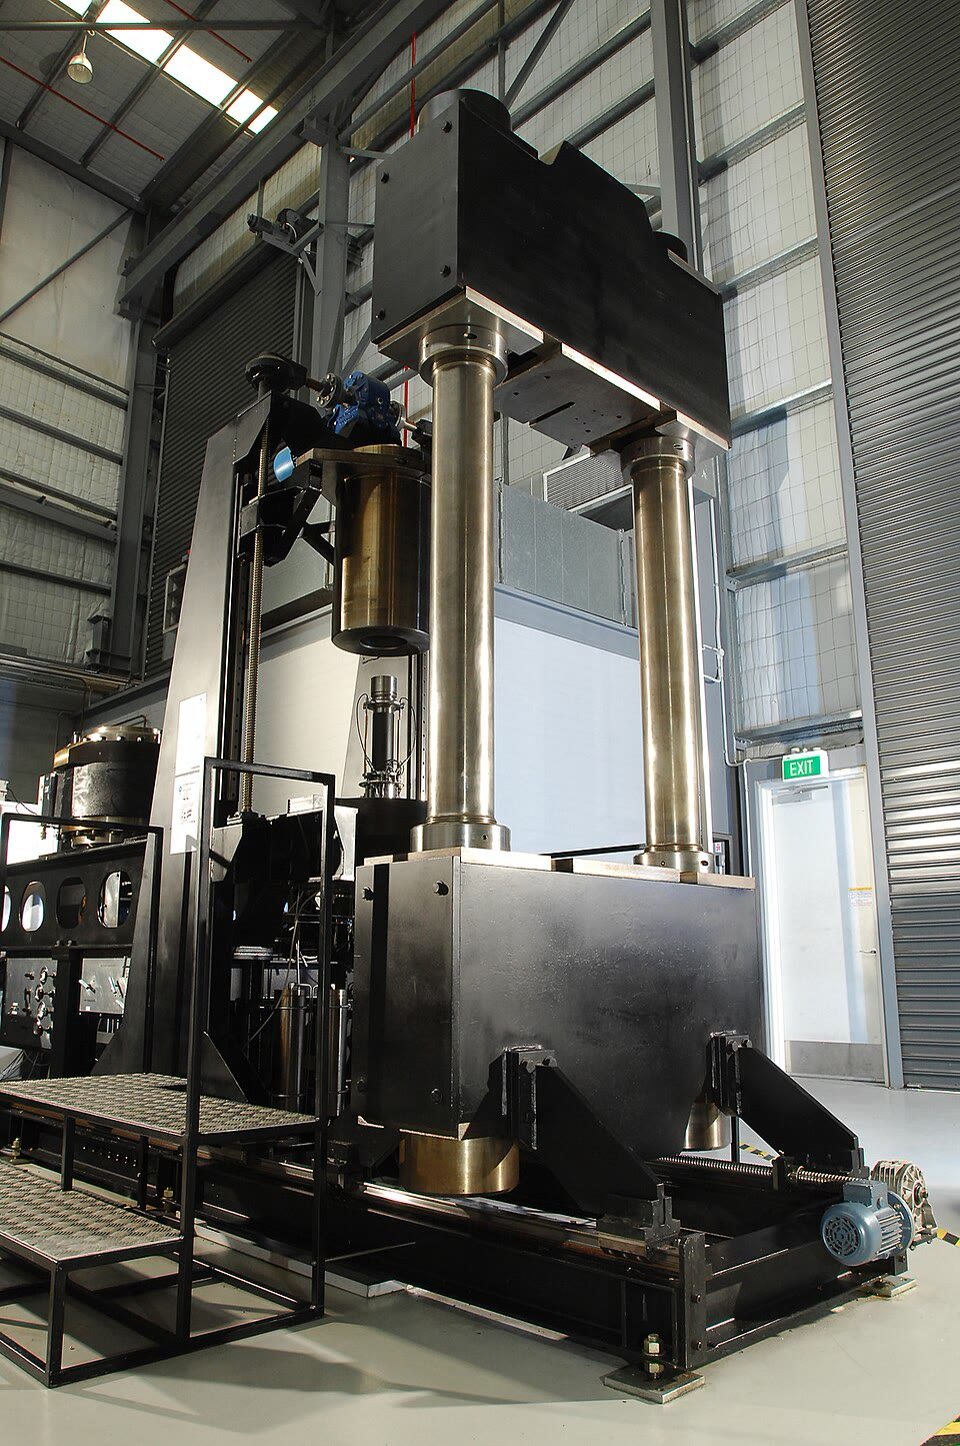
\includegraphics[width=\linewidth]{images/book3/b1-triaxial-cell.jpg}

{\scriptsize Uma célula triaxial de alta pressão para medir a resistência da rocha
(Darryl Peroni, CSIRO, CC BY 3.0).}
% ledger: commons:csiro-triaxial
\end{minipage}
\end{inthelab}

\section{A resistência da litosfera}\label{sec:b1:stress-strain-rheology:envelope}

A cada profundidade a \omterm{def:b1:layered-earth:lithosphere}{litosfera} pode romper-se de duas maneiras: por deslizamento sobre falhas, com uma resistência que cresce com a pressão efetiva, ou por fluência, com uma resistência que cai à medida que ela esquenta. Ela se deforma do modo que exige a menor tensão.

\begin{definition}[Envoltória de resistência, transição frágil--dúctil, camada sismogênica]\label{def:b1:stress-strain-rheology:strength-envelope}
A \emph{envoltória de resistência}\index{envoltória de resistência} da \omterm{def:b1:layered-earth:lithosphere}{litosfera} é a curva, em função da profundidade, da maior \omterm{def:b1:stress-strain-rheology:principal}{tensão diferencial} que ela suporta a uma dada taxa de deformação: a cada profundidade, a menor entre a resistência por atrito e a resistência à fluência. A \emph{transição frágil--dúctil}\index{transição frágil--dúctil} é a profundidade em que as duas são iguais: acima dela a rocha se deforma por falhamento, abaixo por fluência. A \emph{camada sismogênica}\index{camada sismogênica} é a faixa de profundidades em que a maioria dos terremotos começa.
\end{definition}

\begin{proposition}[Resistência por atrito com a profundidade]\label{prop:b1:stress-strain-rheology:brittle-gradient}
Em uma camada de densidade $\rho$ com pressão hidrostática nos poros, uma tensão principal vertical, falhas de toda orientação e nenhuma \omterm{def:b1:stress-strain-rheology:coulomb}{coesão}, com deslizamento
por atrito $\mu$ começa à \omterm{def:b1:stress-strain-rheology:principal}{tensão diferencial}
\begin{align*}
  \sigma_1 - \sigma_3 &= \frac{2\mu}{\sqrt{1+\mu^2} + \mu}\,\rho g z(1-\lambda)
  && \text{se $\sigma_v = \sigma_1$}, \\
  \sigma_1 - \sigma_3 &= \frac{2\mu}{\sqrt{1+\mu^2} - \mu}\,\rho g z(1-\lambda)
  && \text{se $\sigma_v = \sigma_3$},
\end{align*}
com $\lambda = \rho_w/\rho$: o primeiro caso dá falhas normais, o segundo, empurrões.
\end{proposition}

\begin{proof}
A \omterm{def:b1:stress-strain-rheology:lithostatic}{tensão efetiva} vertical é $S = \rho g z - \rho_w g z = \rho g z(1-\lambda)$.
Com $C = 0$ e $k = \sqrt{1+\mu^2}$, o \cref{thm:b1:stress-strain-rheology:failure-angle}
diz que uma falha desliza quando $r = \mu c'/k$, com $r$ o raio e $c'$ o
centro do círculo de Mohr efetivo. Se $\sigma_v = \sigma_1$, então
$\sigma_1' = S$ e $c' = S - r$, logo $rk = \mu S - \mu r$ e
$r = \mu S/(k+\mu)$. Se $\sigma_v = \sigma_3$, então $c' = S + r$ e
$r = \mu S/(k-\mu)$. A \omterm{def:b1:stress-strain-rheology:principal}{tensão diferencial} é $2r$.
\end{proof}

Com $\mu = 0.85$ e $\rho = \qty{2700}{kg.m^{-3}}$, $S$ cresce
\qty{16.7}{MPa} por quilômetro, e a resistência por atrito \qty{13.1}{MPa} por quilômetro sob \omterm{def:b1:stress-strain-rheology:strain}{extensão} e \qty{61.3}{MPa} por
quilômetro sob compressão, quase cinco vezes mais: uma \omterm{def:b1:layered-earth:layers}{crosta} é muito mais fácil de separar do que de empurrar uma contra a outra. Acima de uma \omterm{def:b1:stress-strain-rheology:stress}{tensão normal} efetiva de
\qty{200}{MPa}, o ramo superior da \omterm{prop:b1:stress-strain-rheology:byerlee}{lei de Byerlee} assume, e a inclinação cai, em compressão, para cerca de \qty{35}{MPa} por quilômetro.
% computed in figdata/bachelor-1/strength_envelope.py (tested); ledger: byerlee:1975

\begin{omfigure}
\begin{tikzpicture}
\pgfplotsset{envaxis/.style={omrecord, omdepth, scale only axis, width=5.6cm, height=7.2cm,
  xmin=-1000, xmax=2500, ymin=0, ymax=80, xtick={-1000,0,1000,2000},
  ytick={0,10,...,80}, unbounded coords=jump,
  xlabel={tensão diferencial $\sigma_1-\sigma_3$ (MPa)},
  tick label style={font=\scriptsize}, label style={font=\small},
  scaled x ticks=false, xticklabel style={/pgf/number format/.cd, 1000 sep={\,}}}}
% computed in figdata/bachelor-1/strength_envelope.py; ledger: byerlee:1975, lopez:flow-laws, codata:R, prem:moho-average
\begin{axis}[envaxis, name=cont, ylabel={profundidade (km)}, title={\small (a) continente, \qty{55}{mW.m^{-2}}}]
\addplot[fill=omLithGranite!45, draw=none] table[x=x, y=depth] {figdata/out/bachelor-1-strength_envelope-continental-outline.dat};
\addplot[omThm, line width=0.5pt, restrict x to domain=-1:2450] table[x=thrust, y=depth] {figdata/out/bachelor-1-strength_envelope-continental.dat};
\addplot[omThm, line width=0.5pt, restrict x to domain=-2450:1] table[x expr=-\thisrow{normal}, y=depth] {figdata/out/bachelor-1-strength_envelope-continental.dat};
\addplot[omDef, line width=0.5pt, restrict x to domain=-1:2450] table[x=ductile, y=depth] {figdata/out/bachelor-1-strength_envelope-continental.dat};
\addplot[omDef, line width=0.5pt, restrict x to domain=-2450:1] table[x expr=-\thisrow{ductile}, y=depth] {figdata/out/bachelor-1-strength_envelope-continental.dat};
\addplot[black, line width=1.0pt] table[x=x, y=depth] {figdata/out/bachelor-1-strength_envelope-continental-outline.dat};
\draw[black!60, dashed] (axis cs:-1000,35) -- (axis cs:2500,35);
\node[font=\scriptsize, anchor=south east] at (axis cs:2480,35) {Moho};
\draw[black, densely dotted] (axis cs:0,0) -- (axis cs:0,80);
\draw[black!70] (axis cs:660,13.7) -- (axis cs:1700,18) node[anchor=north, font=\scriptsize, align=center, text=black] {transição\\ \qty{14}{km}};
\draw[black!70] (axis cs:1870,44.6) -- (axis cs:1950,53) node[anchor=north, font=\scriptsize, align=center, text=black] {transição\\ do manto};
\node[font=\scriptsize, anchor=north, omThm] at (axis cs:1500,3) {compressão};
\node[font=\scriptsize, anchor=north, omThm] at (axis cs:-560,3) {extensão};
\node[font=\scriptsize, anchor=west, omDef] at (axis cs:40,31) {quartzo úmido};
\node[font=\scriptsize, anchor=west, omDef] at (axis cs:300,66) {olivina seca};
\end{axis}
\begin{axis}[envaxis, at={(cont.east)}, anchor=west, xshift=0.6cm, yticklabels={}, title={\small (b) fundo oceânico de \qty{60}{Myr}}]
\addplot[fill=omLithBasalt!45, draw=none] table[x=x, y=depth] {figdata/out/bachelor-1-strength_envelope-oceanic-outline.dat};
\addplot[omThm, line width=0.5pt, restrict x to domain=-1:2450] table[x=thrust, y=depth] {figdata/out/bachelor-1-strength_envelope-oceanic.dat};
\addplot[omThm, line width=0.5pt, restrict x to domain=-2450:1] table[x expr=-\thisrow{normal}, y=depth] {figdata/out/bachelor-1-strength_envelope-oceanic.dat};
\addplot[omDef, line width=0.5pt, restrict x to domain=-1:2450] table[x=ductile, y=depth] {figdata/out/bachelor-1-strength_envelope-oceanic.dat};
\addplot[omDef, line width=0.5pt, restrict x to domain=-2450:1] table[x expr=-\thisrow{ductile}, y=depth] {figdata/out/bachelor-1-strength_envelope-oceanic.dat};
\addplot[black, line width=1.0pt] table[x=x, y=depth] {figdata/out/bachelor-1-strength_envelope-oceanic-outline.dat};
\draw[black, densely dotted] (axis cs:0,0) -- (axis cs:0,80);
\draw[black!70] (axis cs:2003,38.2) -- (axis cs:1900,50) node[anchor=north, font=\scriptsize, align=center, text=black] {transição\\ \qty{38}{km}};
\node[font=\scriptsize, anchor=west, omDef] at (axis cs:300,66) {olivina seca};
\end{axis}
\end{tikzpicture}
\par\smallskip{\small \omterm{def:b1:stress-strain-rheology:strength-envelope}{Envoltórias de resistência} à taxa de deformação
\qty{e-15}{s^{-1}}. Vermelho: resistência por atrito pela \omterm{prop:b1:stress-strain-rheology:byerlee}{lei de Byerlee}, com pressão hidrostática nos poros, para compressão (falhamento por empurrão, à direita) e \omterm{def:b1:stress-strain-rheology:strain}{extensão} (falhamento normal, à esquerda, desenhado como negativo); azul: a resistência à fluência do quartzito úmido na \omterm{def:b1:layered-earth:layers}{crosta} continental e da \omterm{def:b1:rock-forming-minerals:groups}{olivina} seca no \omterm{def:b1:layered-earth:layers}{manto}; contorno preto e sombreado: a resistência, a menor das duas em cada profundidade. (a) Um continente com \omterm{def:b1:heat-budget:heat-flow}{fluxo de calor} superficial de \qty{55}{mW.m^{-2}} e uma \omterm{def:b1:layered-earth:layers}{crosta} de \qty{35}{km} de espessura: \omterm{def:b1:layered-earth:layers}{crosta} superior forte, \omterm{def:b1:layered-earth:layers}{crosta} inferior fraca, \omterm{def:b1:layered-earth:layers}{manto} superior forte. (b) Fundo oceânico de \qty{60}{Myr}: uma única camada forte, de \qty{38}{km} de espessura em compressão.}
\label{fig:b1:stress-strain-rheology:envelope}
\end{omfigure}

A figura acima reúne as duas resistências
para duas \omterm{def:b1:layered-earth:lithosphere}{litosferas}. O continente tem a geoterma do \cref{ch:b1:heat-budget} com um \omterm{def:b1:heat-budget:heat-flow}{fluxo de calor} superficial de \qty{55}{mW.m^{-2}}, uma \omterm{def:b1:layered-earth:layers}{crosta} de quartzito úmido com \qty{35}{km} de espessura e \omterm{def:b1:rock-forming-minerals:groups}{olivina} seca abaixo; o fundo oceânico tem \qty{60}{Myr}, com a geoterma de semiespaço do mesmo capítulo, e \omterm{def:b1:rock-forming-minerals:groups}{olivina} desde o fundo do mar para baixo. A taxa de deformação é
\qty{e-15}{s^{-1}}. Os \qty{35}{km} são a profundidade média do \omterm{def:b1:layered-earth:discontinuity}{Moho} sob os continentes no modelo de Terra de referência do \cref{ch:b1:layered-earth}.
% ledger: prem:moho-average

Sob o continente, a \omterm{def:b1:stress-strain-rheology:strength-envelope}{transição frágil--dúctil} cai a \qty{13.7}{km} em compressão, a \qty{249}{\degreeCelsius}, e a \qty{17.1}{km} em \omterm{def:b1:stress-strain-rheology:strain}{extensão}. Uma \omterm{def:b1:layered-earth:layers}{crosta} mais quente a faria subir, e uma mais fria a empurraria para baixo, pois a lei de fluência depende apenas da temperatura, para uma dada tensão. A transição é o nível mais forte da \omterm{def:b1:layered-earth:layers}{crosta}.
Abaixo dela, a resistência desaba: no \omterm{def:b1:layered-earth:discontinuity}{Moho}, a \qty{527}{\degreeCelsius}, o quartzito flui sob \qty{7.6}{MPa}, enquanto a \omterm{def:b1:rock-forming-minerals:groups}{olivina}, à mesma temperatura, precisaria de cerca de \qty{30000}{MPa}, tão além da resistência por atrito que o topo do \omterm{def:b1:layered-earth:layers}{manto} volta a ser frágil. Uma segunda transição segue a \qty{44.6}{km} em compressão. A \omterm{def:b1:layered-earth:layers}{crosta} inferior deste modelo é uma camada mole entre duas fortes: o ``sanduíche de geleia''. Sob o oceano, a \omterm{def:b1:layered-earth:lithosphere}{litosfera} inteira é \omterm{def:b1:rock-forming-minerals:groups}{olivina}, e a resistência cresce até uma única transição a \qty{38.2}{km}, a \qty{641}{\degreeCelsius}.
% computed in figdata/bachelor-1/strength_envelope.py (tested)

Os terremotos concordam com a envoltória oceânica: dentro das placas oceânicas, eles atingem profundidades onde a temperatura é
\qtyrange{600}{800}{\degreeCelsius}, perto dos \qty{641}{\degreeCelsius} da transição única do modelo. Terremotos mais profundos ocorrem apenas onde uma placa afunda sob outra, até mais de \qty{700}{km}
(\cref{ch:b1:active-margins}).
% ledger: jackson:jelly, usgs:deepest

O \omterm{def:b1:layered-earth:layers}{manto} continental é onde o quadro é disputado. Por cerca de vinte anos, o sanduíche de geleia foi a visão predominante, construída sobre medidas de laboratório de \omterm{def:b1:rock-forming-minerals:groups}{olivina} seca e sobre alguns terremotos que se pensava estarem abaixo do \omterm{def:b1:layered-earth:discontinuity}{Moho}. Em 2002, James Jackson argumentou que ela deveria ser abandonada: profundidades melhores mostraram que os terremotos dos continentes se confinam a uma única camada, em geral a \omterm{def:b1:layered-earth:layers}{crosta} superior, às vezes a \omterm{def:b1:layered-earth:layers}{crosta} inteira, sem terremotos convincentes no \omterm{def:b1:layered-earth:layers}{manto} abaixo, mesmo onde o \omterm{def:b1:layered-earth:discontinuity}{Moho} está a apenas \qtyrange{300}{500}{\degreeCelsius}. Pequenas quantidades de água, algumas partes por milhão em \omterm{def:b1:rock-forming-minerals:groups}{olivina}, bastam para enfraquecê-la dramaticamente, e o \omterm{def:b1:layered-earth:layers}{manto} continental pode muito bem conter tanto; a resistência dos continentes estaria então sobretudo em sua \omterm{def:b1:layered-earth:layers}{crosta}. As duas visões desenham envoltórias diferentes a partir das mesmas leis, com \omterm{def:b1:rock-forming-minerals:groups}{olivina} seca ou úmida abaixo do \omterm{def:b1:layered-earth:discontinuity}{Moho}.
% ledger: jackson:jelly
Qualquer que seja a visão certa, uma envoltória é um limite e não uma medida: as leis de laboratório são extrapoladas por muitas ordens de grandeza da taxa de deformação, e os picos de tensão que ela mostra, acima de um gigapascal, estão muito acima dos \qtyrange{1}{10}{MPa} que os terremotos são vistos liberando.
% ledger: jackson:jelly

\section{Exercícios}

\begin{exercise}[$\star$]\label{exo:b1:stress-strain-rheology:1}
Tome uma \omterm{def:b1:layered-earth:layers}{crosta} de densidade \qty{2700}{kg.m^{-3}} e $g = \qty{9.81}{m.s^{-2}}$. À profundidade de \qty{10}{km}, calcule (a) a tensão vertical, (b) a pressão hidrostática nos poros, (c) a \omterm{def:b1:stress-strain-rheology:lithostatic}{tensão efetiva} vertical e a razão de pressão nos poros
$\lambda$.
\end{exercise}

\begin{exercise}[$\star$]\label{exo:b1:stress-strain-rheology:2}
(a) Uma camada de \qty{10}{km} de comprimento é esticada até \qty{13}{km}: dê sua \omterm{def:b1:stress-strain-rheology:strain}{extensão} e seu \omterm{def:b1:stress-strain-rheology:strain}{alongamento}. (b) Outra, de \qty{10}{km} de comprimento, é encurtada até \qty{7}{km}. (c) Duas linhas de uma rocha que eram perpendiculares agora formam um ângulo de \ang{60}: quais são o cisalhamento angular e a \omterm{def:b1:stress-strain-rheology:strain}{deformação de cisalhamento}?
\end{exercise}

\begin{exercise}[$\star$]\label{exo:b1:stress-strain-rheology:3}
Em um ponto, $\sigma_1 = \qty{100}{MPa}$ e $\sigma_3 = \qty{40}{MPa}$.
(a) Desenhe o círculo de Mohr. (b) Qual é a maior tensão de cisalhamento, em quais planos ela atua, e que \omterm{def:b1:stress-strain-rheology:stress}{tensão normal} atua sobre eles? (c) Calcule $\sigma_n$
e $\tau$ sobre o plano cuja normal faz \ang{30} com $\sigma_1$.
\end{exercise}

\begin{exercise}[$\star$]\label{exo:b1:stress-strain-rheology:4}
Uma rocha tem \omterm{def:b1:stress-strain-rheology:coulomb}{coesão} \qty{10}{MPa} e \omterm{def:b1:stress-strain-rheology:coulomb}{ângulo de atrito interno}
\ang{30}. (a) Em que ângulo com $\sigma_1$ ela se rompe, e que ângulo formam entre si os dois planos de fratura possíveis? (b) Com
$\sigma_3' = \qty{20}{MPa}$, qual $\sigma_1'$ efetivo a rompe?
\end{exercise}

\begin{exercise}[$\star\star$]\label{exo:b1:stress-strain-rheology:5}
Nos eixos $x$ (horizontal) e $y$ (vertical), $\sigma_{xx} = \qty{60}{MPa}$,
$\sigma_{yy} = \qty{20}{MPa}$ e $\sigma_{xy} = \qty{15}{MPa}$. (a) Calcule as
\omterm{def:b1:stress-strain-rheology:principal}{tensões principais} e o ângulo $\theta_p$. (b) Verifique com a
\cref{prop:b1:stress-strain-rheology:transformation} que o plano de normal
$\theta_p$ não carrega tensão de cisalhamento e que tem a \omterm{def:b1:stress-strain-rheology:stress}{tensão normal} $\sigma_1$. (c) Qual é a
maior tensão de cisalhamento neste ponto?
\end{exercise}

\begin{exercise}[$\star\star$]\label{exo:b1:stress-strain-rheology:6}
Uma zona de cisalhamento deformou sua rocha por um \omterm{def:b1:stress-strain-rheology:shear-types}{cisalhamento simples} $\gamma = 2$. (a) Calcule
os \omterm{def:b1:stress-strain-rheology:strain}{alongamentos} principais e o ângulo do eixo longo da \omterm{def:b1:stress-strain-rheology:strain-ellipse}{elipse de deformação} com a direção de cisalhamento. (b) Verifique que a área não mudou. (c) Uma linha de material estava a \ang{45} da direção de cisalhamento, subindo no sentido do cisalhamento: onde ela está agora, e qual é seu \omterm{def:b1:stress-strain-rheology:strain}{alongamento}? Compare com (a).
\end{exercise}

\begin{exercise}[$\star\star$]\label{exo:b1:stress-strain-rheology:7}
Numa zona de cisalhamento de \qty{200}{m} de espessura, pequenas manchas arredondadas em uma ardósia tornaram-se elipses com eixos na razão 4 para 1. Suponha um \omterm{def:b1:stress-strain-rheology:shear-types}{cisalhamento simples}, sem mudança de área. (a) Encontre $S_1$, $S_2$ e $\gamma$. (b) Em que ângulo com as paredes da zona devem jazer os eixos longos? (c) Quanto uma parede se deslocou além da outra?
\end{exercise}

\begin{exercise}[$\star\star$]\label{exo:b1:stress-strain-rheology:8}
Uma falha a \qty{3}{km} de profundidade, em \omterm{def:b1:layered-earth:layers}{crosta} de densidade \qty{2700}{kg.m^{-3}}, suporta a \omterm{def:b1:stress-strain-rheology:stress}{tensão normal} de \qty{70}{MPa} e a tensão de cisalhamento de \qty{30}{MPa}. (a) Com pressão hidrostática nos poros, ela desliza segundo a \omterm{prop:b1:stress-strain-rheology:byerlee}{lei de Byerlee}? (b) E se os poros forem selados e $\lambda = 0.6$? (c) Encontre o valor de $\lambda$ a partir do qual ela começa a deslizar.
\end{exercise}

\begin{exercise}[$\star\star$]\label{exo:b1:stress-strain-rheology:9}
Use a lei de fluência do quartzito úmido (\cref{prop:b1:stress-strain-rheology:creep}). (a) De que fator a tensão deve subir para que ele flua dez vezes mais depressa? (b) De que fator sua resistência cai entre \qty{400}{\degreeCelsius}
e \qty{500}{\degreeCelsius}, à mesma taxa e com $V = 0$? (c) Explique com esses dois resultados por que a profundidade da \omterm{def:b1:stress-strain-rheology:strength-envelope}{transição frágil--dúctil}
depende muito mais do \omterm{def:b1:heat-budget:geotherm}{geotermo} do que da taxa de deformação.
\end{exercise}

\begin{exercise}[$\star\star\star$]\label{exo:b1:stress-strain-rheology:10}
Onde a tensão vertical é $\sigma_2$, as falhas são transcorrentes. Suponha que a \omterm{def:b1:stress-strain-rheology:lithostatic}{tensão efetiva} vertical seja então a média $(\sigma_1' + \sigma_3')/2$.
(a) Mostre que o deslizamento com atrito $\mu$ e sem \omterm{def:b1:stress-strain-rheology:coulomb}{coesão} começa em $\sigma_1 - \sigma_3 = 2\mu\,\rho g z(1-\lambda)/\sqrt{1+\mu^2}$. (b) Calcule a inclinação em megapascals por quilômetro para $\mu = 0.85$ e $\rho = \qty{2700}{kg.m^{-3}}$, e situe-a entre as inclinações das falhas normais e dos empurrões. (c) Exprima cada uma das três inclinações como múltiplo da \omterm{def:b1:stress-strain-rheology:lithostatic}{tensão efetiva} vertical.
\end{exercise}

\begin{exercise}[$\star\star\star$]\label{exo:b1:stress-strain-rheology:11}
Modele a \omterm{def:b1:layered-earth:lithosphere}{litosfera} oceânica de \qty{60}{Myr} como um semiespaço resfriado a partir de \qty{1350}{\degreeCelsius}, com a superfície a \qty{0}{\degreeCelsius} e
$\kappa = \qty{e-6}{m^2.s^{-1}}$: $T = \num{1350}\operatorname{erf}\bigl(z/(2\sqrt{\kappa t})\bigr)$.
(a) Calcule $2\sqrt{\kappa t}$. (b) Encontre as profundidades das isotermas de
\qty{600}{\degreeCelsius} e \qty{800}{\degreeCelsius}. (c) Os terremotos
dentro das placas oceânicas atingem as profundidades onde a temperatura está entre
\qtyrange{600}{800}{\degreeCelsius}. Compare com a \omterm{def:b1:stress-strain-rheology:strength-envelope}{transição frágil--dúctil} da \omterm{def:b1:stress-strain-rheology:strength-envelope}{envoltória de resistência} oceânica deste capítulo, a
\qty{38.2}{km} e \qty{641}{\degreeCelsius}.
% ledger: jackson:jelly
\end{exercise}

\begin{exercise}[$\star\star\star$]\label{exo:b1:stress-strain-rheology:12}
Uma rocha é cortada por fraturas de toda orientação, todas contendo a direção de $\sigma_2$, com \omterm{def:b1:stress-strain-rheology:coulomb}{coesão} nula e atrito 0.85. As \omterm{def:b1:stress-strain-rheology:principal}{tensões principais} efetivas são $\sigma_1' = \qty{110}{MPa}$ e
$\sigma_3' = \qty{20}{MPa}$. (a) Mostre que algumas fraturas deslizam. (b) Encontre a faixa do ângulo entre as fraturas que deslizam e $\sigma_1$. Qual delas está no meio da faixa? (c) Até que valor de $\sigma_1'$, com $\sigma_3'$ fixo, ao menos uma fratura ainda desliza?
\end{exercise}

\section{Problema: a falha desliza?}

\begin{problem}[{Problema de fim de semana --- a tensão sobre uma falha normal a cinco quilômetros de profundidade, sua margem de segurança e a elevação da pressão nos poros que a faria deslizar}]
\label{pb:b1:stress-strain-rheology:1}
% values: calc/ch16.py; ledger: byerlee:1975, hb81:denver
Uma falha tem \omterm{def:b1:geological-maps:attitude}{direção} norte--sul e mergulha \ang{60} para leste. Um poço de descarte atinge a falha a uma profundidade de \qty{5.00}{km}, em \omterm{def:b1:layered-earth:layers}{crosta} de densidade
\qty{2700}{kg.m^{-3}} cujos poros se conectam à superfície. Uma medida no poço dá a tensão horizontal perpendicular à falha,
\qty{75.0}{MPa}; a tensão horizontal ao longo da \omterm{def:b1:geological-maps:attitude}{direção} fica entre ela e a tensão vertical, de modo que o problema é bidimensional no plano vertical leste--oeste. Tome $g = \qty{9.81}{m.s^{-2}}$, água de densidade
\qty{1000}{kg.m^{-3}} e a \omterm{prop:b1:stress-strain-rheology:byerlee}{lei de Byerlee}. Dê as tensões com
\qty{0.01}{MPa}.

\medskip
\noindent\textbf{Parte I --- O estado de tensão.}
\begin{enumerate}
  \item Calcule a tensão vertical na profundidade da falha.
  \item Calcule a pressão hidrostática nos poros ali, e a razão $\lambda$.
  \item Qual das duas tensões é $\sigma_1$ e qual é $\sigma_3$? Que tipo de falha esse estado de tensão impulsiona?
  \item Calcule a \omterm{def:b1:stress-strain-rheology:principal}{tensão diferencial}, o centro e o raio do círculo de Mohr.
  \item Calcule as \omterm{def:b1:stress-strain-rheology:principal}{tensões principais} efetivas e o centro do círculo efetivo.
  \item Com $x$ horizontal para leste e $y$ vertical, escreva as três componentes $\sigma_{xx}$, $\sigma_{yy}$, $\sigma_{xy}$. Por que $\sigma_{xy}$ é nula?
\end{enumerate}

\medskip
\noindent\textbf{Parte II --- As tensões na falha.}
\begin{enumerate}[resume]
  \item Dê o vetor unitário normal à falha nos eixos da questão 6, e o ângulo $\theta$ entre ele e $\sigma_1$.
  \item Calcule $\sigma_n$ e $\tau$ na falha com
        \cref{prop:b1:stress-strain-rheology:transformation}.
  \item Verifique os dois valores com o círculo de Mohr: a partir da extremidade $\sigma_1$, em que ângulo jaz a falha?
  \item Calcule a \omterm{def:b1:stress-strain-rheology:stress}{tensão normal} efetiva sobre a falha.
  \item Calcule a razão $\tau/\sigma_n'$ e compare-a com 0.85.
  \item Que tensão de cisalhamento faria a falha deslizar sob a \omterm{def:b1:stress-strain-rheology:stress}{tensão normal} efetiva atual? Em quantos megapascals ela fica aquém disso?
\end{enumerate}

\medskip
\noindent\textbf{Parte III --- O círculo de Mohr e a lei de Byerlee.}
\begin{enumerate}[resume]
  \item Desenhe o círculo de Mohr efetivo e a reta de Byerlee em escala.
  \item Calcule a distância do centro do círculo à reta e compare-a com o raio. Algum plano que passe pela rocha pode deslizar?
  \item Qual plano deslizaria primeiro? Dê seu ângulo com $\sigma_1$ e seu \omterm{def:b1:geological-maps:attitude}{mergulho}.
  \item Com a \cref{prop:b1:stress-strain-rheology:brittle-gradient}, calcule a \omterm{def:b1:stress-strain-rheology:principal}{tensão diferencial} na qual falhas normais deslizam a esta profundidade, e confira-a com a inclinação de \qty{13.1}{MPa} por quilômetro.
  \item Quão baixa teria de cair a tensão horizontal para que o plano mais bem orientado deslizasse?
  \item Quão baixa teria de cair a tensão horizontal para que a falha do problema deslizasse? Explique por que ela é mais baixa.
\end{enumerate}

\medskip
\noindent\textbf{Parte IV --- Injeção.}
\begin{enumerate}[resume]
  \item Explique por que uma elevação $\Delta P$ da pressão nos poros desloca o círculo efetivo de $\Delta P$ para a esquerda sem mudar seu raio.
  \item Calcule a elevação da pressão nos poros que leva o plano mais bem orientado a deslizar.
  \item O poço está cheio de água. Que pressão extra a bomba deve aplicar na boca do poço para elevar a pressão nos poros na falha por essa quantidade? A que altura de coluna de água ela equivale?
  \item Se o atrito na falha fosse 0.6 em vez de 0.85, ela já estaria deslizando? O que o silêncio da falha diz sobre seu atrito?
  \item Em que razão $\lambda$ o plano mais bem orientado desliza?
  \item Com uma casa decimal, em megapascals, que elevação da pressão nos poros leva esta falha a deslizar?
\end{enumerate}
\end{problem}
